\chapter{関連研究}
心理学的時間の関連研究や用語の定義,及びアプリケーションの先行事例を示す.

\section{時間の定義と心理的時間について}
時間は出来事や変化を認識する為の基礎的な概念である.芸術,哲学,自然科学,心理学を始めとした複合的な分野で議論されるテーマであるが,ここでは心理学的観点から述べる.心理学では我々の認識世界には2種類の時間が推移しているとされている.1つは客観的時間・物理的時間であり,時計等で表される誰もが客観的に認められる時間である.2つ目は主観的・心理的時間であり,主観的に推移する意識の上での時間の流れである.心理的時間とは,何らかの出来事の生起からどのくらいの長さで時間が経過するか,あるいはどれくらいの時間が過ぎたかという内的経験である\cite{Meck2005}.心理的時間を対象とした研究では,5 秒以内の持続時間を時間知覚,それ以上持続する時間の体験は,時間評価と定義する事がある為\cite{加藤2005},ここでは時間評価という用語を用いる.

\section{時間評価について}
本研究の時間評価の定義は「心理的現在を超えた経過時間に対して,それを長い,短いと感じること,あるいは常用時間単位と結びつけて,何分ぐらい経ったと思うこと,あるいは,ある持続時間(または時間間隔)と別な持続時間 (または時間間隔)を比較して,どちらが(どれくらい)長いと判断すること,これらの心的働きと行為」とする\cite{松田2009a}.時間評価に影響を与える要因として複合的な関与が考えられている.代表的な要因は生物学的・生理的要因\footnote{例えば心拍数\cite{松田堀江一川2011}\cite{松田一川橘2015},体温\cite{松田堀江一川2011}\cite{Hoagland1933},血圧\cite{松田堀江一川2011},年齢\cite{Espinosa2003}\cite{一川2009a}\cite{加藤宮澤多田 2006} \cite{和田村田2001}などが挙げられる.},認知的要因,パーソナリティ要因\footnote{例えば,Type A\cite{Burnam1975}\cite{折原1993}\cite{折原1995},性格特性\cite{新井1985}\cite{Bell1972}\cite{Campos1966}\cite{Eysenck1959}\cite{今井1965}\cite{岩脇1959}\cite{加藤1967}\cite{Rammsayer1997} \cite{RammsayerRammstedt2000}\cite{ReedKenna1964}\cite{Wudel1979},不安\cite{Bar-Haim2010}\cite{Hare1963}\cite{村中坂野2000}などがある.}に分類が可能である.
特に認知的要因には,刺激のまとまり\cite{松田1965},刺激頻度\cite{松田1967},色\cite{勝浦2007},時間経過への注意\cite{藤原狩野1994},刺激の大きさ\cite{Ono2007}\cite{Thomas1975},課題の難易度\cite{島村篠原長山1991}\cite{篠原2009}などが考えられている.
時間評価の研究方法には,ターゲットとなる時間の長さを秒,分,時間などの単位で評価者に言語などで示し,その時間の長さと感じられる時間だけボタンなどを押させる方法である産出法,基準となる時間の長さを視覚刺激などで提示した後にそれと同じ時間の長さをボタン押しなどで産出させる方法である再生法,何らかの課題を実施した後,その課題に要した時間の長さを秒,分,時間などの単位で答える方法である言語的見積もり法,などがある\cite{一川2008}\footnote{産出法は作成法,言語的見積もり法は言語的評価や評価法とも呼ばれる.}.尚,結果表記において,「過大評価」と「過小評価」と評価する.「過大評価」と「過小評価」の評価方法は研究手法によって様々だが\cite{松田1985}\cite{篠原1996}\cite{加藤宮澤多田2006}本研究において「過大評価」は客観的な時間よりも心理的時間が長くなること,「過小評価」は客観的な時間よりも短くなることと定義する.

\section{遅刻について}
社会生活を送るにあたり事前に開始時刻や日程等が決められている行為への参加に遅れる場合がある.我々はこの事象を「遅刻」と定義しており,相手に対し自らの評価を下げる要因の一つとして回避すべき課題としている.遅刻に対する許容範囲は個人差\cite{drill}や文化差\footnote{例えば列車においてイタリアやフランスは15分以上,イギリスでは10分以上,ドイツでは5分以上の遅延で「遅刻」の対象となるとされている\cite{train}.}に左右されるが,近代における日本は厳しい傾向にある\cite{delay}.

\section{日常生活動作について}
日常生活動作(Activities of Daily Living;ADL)とは,人が日常生活において繰り返す,身の回りの活動や動作のことである.具体的には,身の回りの動作(食事,更衣,整容,排泄,入浴の各動作),移動動作,その他生活関連動作(家事動作,交通機関の利用等)を指す\cite{酒井2003}.我々は外出準備に平均1時間程度日常生活動作を複数こなしている\cite{duhouse}.本研究では「起床時から外出時刻までに外出準備として行われる日常生活動作」とする.

\section{アプリケーションに関して}
今日朝を始めとした日常生活動作に関するiOSアプリケーションが開発されている.例えば「あさとけい」は朝の起床時間〜外出時間までの準備時間を対象にしたアプリケーションであり,登録した出発時刻に対するカウントダウン機能がある\cite{あさとけい}また,「たすくま」はタスクシュート式\footnote{タスクシュートは大橋悦夫が開発した管理手法であり,1日の仕事を直列に並べ,見積時間を出すと終了時刻を自動予測するシステムを用いて行われる.}のタスク管理アプリである\cite{たすくま}.「たすくま」はタスク毎の時間を記録すると,予測タスクの自動生成が行われ,日常生活動作を始めとしたルーティンワークの予測が行われる.ルーチンタイマーは複数タスクを「ルーチン」として登録し,設定した所要時間をもとに一つ一つアナウンスされるアプリケーションである\cite{ルーチンタイマー}.ルーチンタイマーの導入によって対象のルーティンワークの可視化や登録したタスク別終了予定時刻の把握が可能である.しかし,実際の行動を計測し,個人に最適化されたリマインダーを用いて注意力を向上させるアプリケーションはまだ開発されていない.

\begin{figure}[ht]
\begin{center}
\begin{tabular}{c}

	\begin{minipage}[b]{0.5\linewidth}
	\begin{center}
		\fbox{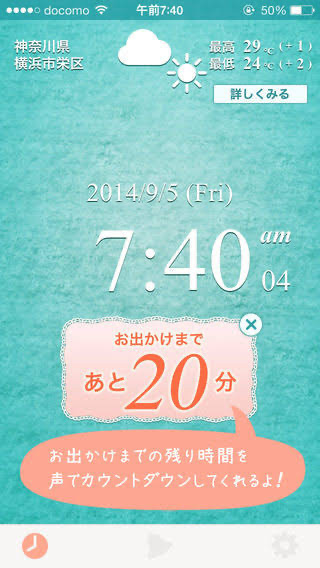
\includegraphics[width=5cm]{images/2/asa1.jpg}}
		\caption{あさとけいカウントダウン}
		\label{fig:top_point}
	\end{center}
  	\end{minipage}

  	\begin{minipage}[b]{0.5\linewidth}
	\begin{center}
		\fbox{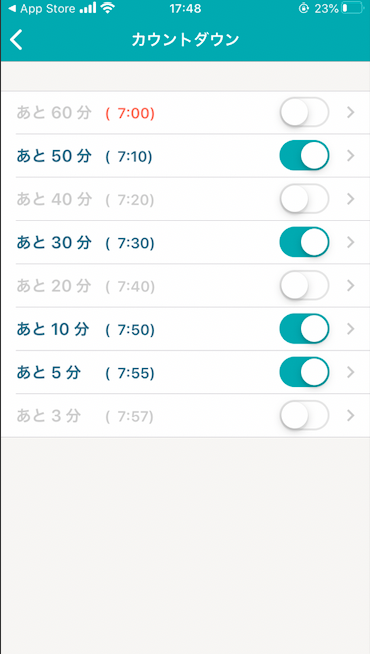
\includegraphics[width=5cm]{images/2/asa2.png}}
		\caption{あさとけいタスク登録}
		\label{fig:top_ranking}
	\end{center}
  	\end{minipage}

  	\\

  	\begin{minipage}[b]{0.5\linewidth}
	\begin{center}
		\fbox{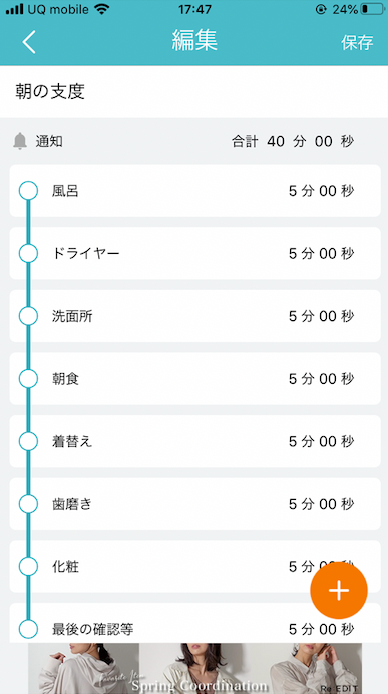
\includegraphics[width=5cm]{images/2/routine1.png}}
		\caption{ルーティンワークカウントダウン}
		\label{fig:goal_alert}
	\end{center}
  	\end{minipage}

  	\begin{minipage}[b]{0.5\linewidth}
	\begin{center}
		\fbox{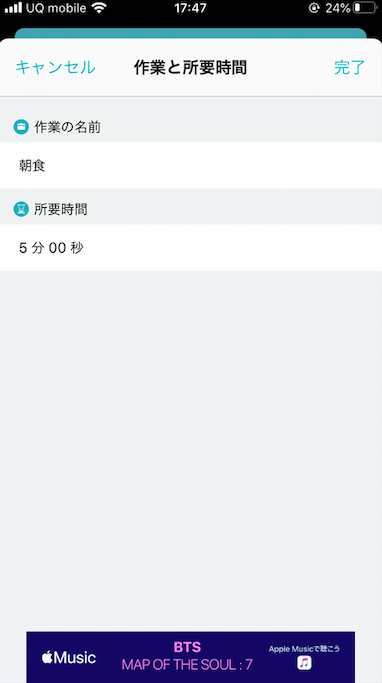
\includegraphics[width=5cm]{images/2/routine2.png}}
		\caption{ルーティンワークカウントダウン}
		\label{fig:top_goal}
	\end{center}
  	\end{minipage}

\end{tabular}
\end{center}
\end{figure}


\section{まとめ}
本章では,本研究における関連研究を整理し,問題意識を洗い出した.
次章では,筆者が本研究に先立ち行った研究について述べ,問題意識を洗い出す.